\scanpage{362}
\uuline{Formule de Decalage} (Quillen - Bousfield) [cf thèse Illusie].
\mspage{1}

\deleted{$F$}
\[
L_*F(M,n)\qquad L_*F(M[n])
\]
\deleted{\[
\begin{gathered}
L_i\operatorname{Sym}^{\unsure{j|i}}(M,n)\simeq L_{i+n}\Lambda^j(M,n+1)\\
L_i\Lambda^j(M,n)\simeq L_{i+n}\Gamma^j(M,n+1)
\end{gathered}
\]}
\margin{\diagram{\begin{tikzcd}\underbrace{M}\arrow[r]&\underbrace{M}\end{tikzcd}}}
\deleted{$L_i\operatorname{Sym}^j\unsure{(M,n)}\Longrightarrow L_{i+n}\Lambda^j$}
\diagram{\begin{tikzcd}
K(M,n)\arrow[r]&E(M,n+1)\arrow[d,no head]\\
&K(M,n+1)
\end{tikzcd}}
\[
\begin{gathered}
\operatorname{Sym}K(M,n)\otimes\Lambda E(M,n+1).\\
\Lambda^{n+1}\Phi\otimes_{\mathbb Z}M
\end{gathered}
\]
\diagram{\begin{tikzcd}[column sep=small]
0\arrow[r]&\operatorname{Sym}^i\underline{K(M,n)}\arrow[r]&\operatorname{Sym}^{i-1}K(M,n)\otimes\Lambda^1\underline{\underline{E(M,n+1)}}\arrow[r]&\operatorname{Sym}^{i-2}K(M,n)\otimes\Lambda^2\underline{E(M,n+1)}\\
&&{}\arrow[r]&\Lambda^iE(M,n+1)\arrow[r]&\Lambda^iK(M,n+1)\arrow[dr,bend right=15]\\
&&&&&0
\end{tikzcd}}
\diagram{\begin{tikzcd}[column sep=small]
0\arrow[r]&\Lambda^iK(M,n)\arrow[r]&\Lambda^{i-1}K(M,n)\otimes\operatorname{Sym}^1E(M,n+1)\arrow[r]&\ldots\operatorname{Sym}^iE(M,n+1)\arrow[d,bend right=10]\\
&&&\operatorname{Sym}^iK(M,n+1)\arrow[dr,bend right=15]\\
&&&&0
\end{tikzcd}}
\diagram{\begin{tikzcd}[column sep=small]
0\arrow[r]&\Gamma^iK(M,n)\arrow[r]&\Gamma^{i-1}K(M,n)\otimes\Lambda^{i}E(\ldots)
\end{tikzcd}}
\figure{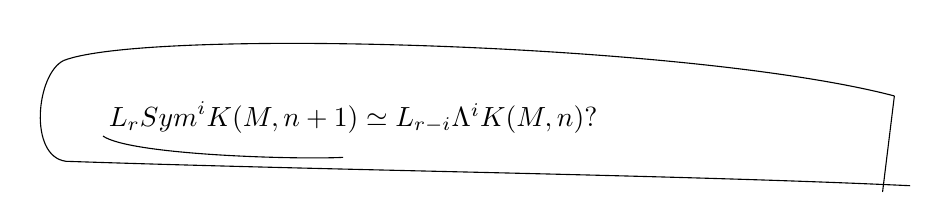
\begin{tikzpicture}
\node[anchor=west] at (-5,0) {$L_r\operatorname{Sym}^i K(M,n+1)\simeq L_{r-i}\Lambda^i K(M,n)\unsure{?}$};
\draw (-5.45,.72) .. controls (-4.4,1.13) and (2.5,.95) .. (5.1,.27);
\draw (5.1,.27)--(4.95,-.95);
\draw (-5.45,.72) .. controls (-5.8,.55) and (-5.9,-.5) .. (-5.42,-.56)
 .. controls (-1.9,-.68) and (2.3,-.73) .. (5.3,-.87);
\draw (-4.95,-.24) .. controls (-4.6,-.48) and (-2.5,-.54) .. (-1.9,-.51);
\end{tikzpicture}}
\[
\begin{gathered}
L_*\operatorname{Sym}^iX[1]\simeq L_{*\deleted{-i}}\Lambda^iX[-i]\\
L_*\Lambda^i(X[1])\simeq L_*\Gamma^iX[-i]\\
L_*\operatorname{Sym}^iX[2]\simeq L_*\Gamma^iX[-2i]
\end{gathered}
\]
\figure{\begin{tikzpicture}\draw (0,0)--(.1,0);\end{tikzpicture}}
\mspage{363}
